%%%%%%%%%%%%%%%%%%%%%%%%%%%%%%%%%%%%%%%%%%%%%%%%%%%%%%%%%%%%%%%%
% %
% Seth Cram %
% ECE351 Section 53 %
% Lab Number 3 %
% Due 02/08/2022 %
% Any other necessary information needed to navigate the file %
%
%
% %
%%%%%%%%%%%%%%%%%%%%%%%%%%%%%%%%%%%%%%%%%%%%%%%%%%%%%%%%%%%%%%%%
%%%%%%%%%%%%%%%%%%%%%%%%%%%%%%%%%%%%%%%%%%%
%%% DOCUMENT PREAMBLE %%%
\documentclass[12pt]{report}
\usepackage[english]{babel}
%\usepackage{natbib}
\usepackage{url}
\usepackage[utf8x]{inputenc}
\usepackage{amsmath}
\usepackage{graphicx}
\graphicspath{{images/}}
\usepackage{parskip}
\usepackage{fancyhdr}
\usepackage{vmargin}
\usepackage{listings}
\usepackage{hyperref}
\usepackage{xcolor}
\usepackage{verbatim}

\definecolor{codegreen}{rgb}{0,0.6,0}
\definecolor{codegray}{rgb}{0.5,0.5,0.5}
\definecolor{codeblue}{rgb}{0,0,0.95}
\definecolor{backcolour}{rgb}{0.95,0.95,0.92}

\begin{comment} %have to use verbatim package for this

\section{Personal Notes}
            


\end{comment}

\lstdefinestyle{mystyle}{
    backgroundcolor=\color{backcolour},   
    commentstyle=\color{codegreen},
    keywordstyle=\color{codeblue},
    numberstyle=\tiny\color{codegray},
    stringstyle=\color{codegreen},
    basicstyle=\ttfamily\footnotesize,
    breakatwhitespace=false,         
    breaklines=true,                 
    captionpos=b,                    
    keepspaces=true,                 
    numbers=left,                    
    numbersep=5pt,                  
    showspaces=false,                
    showstringspaces=false,
    showtabs=false,                  
    tabsize=2
}
 
\lstset{style=mystyle}

\setmarginsrb{3 cm}{2.5 cm}{3 cm}{2.5 cm}{1 cm}{1.5 cm}{1 cm}{1.5 cm}

\title{Lab 3}		%TITLE						
% Title
\author{ Seth Cram}						
% Author
\date{01/30/2022}
% Date

\makeatletter
\let\thetitle\@title
\let\theauthor\@author
\let\thedate\@date
\makeatother

\pagestyle{fancy}
\fancyhf{}
\rhead{\theauthor}
\lhead{\thetitle}
\cfoot{\thepage}
%%%%%%%%%%%%%%%%%%%%%%%%%%%%%%%%%%%%%%%%%%%%
\begin{document}

%%%%%%%%%%%%%%%%%%%%%%%%%%%%%%%%%%%%%%%%%%%%%%%%%%%%%%%%%%%%%%%%%%%%%%%%%%%%%%%%%%%%%%%%%

\begin{titlepage}
	\centering
    \vspace*{0.5 cm}
   % \includegraphics[scale = 0.075]{bsulogo.png}\\[1.0 cm]	% University Logo
\begin{center}    \textsc{\Large   ECE 351 - 53 }\\[2.0 cm]	\end{center}% University Name
	\textsc{\Large Discrete Convolution }\\[.5 cm]				% Course Code
	\rule{\linewidth}{0.2 mm} \\[0.4 cm]
	{ \huge \bfseries \thetitle}\\
	\rule{\linewidth}{0.2 mm} \\[1.5 cm]
	
	\begin{minipage}{0.4\textwidth}
		\begin{flushleft} \large
		%	\emph{Submitted To:}\\
		%	Name\\
          % Affiliation\\
           %contact info\\
			\end{flushleft}
			\end{minipage}~
			\begin{minipage}{0.4\textwidth}
            
			\begin{flushright} \large
			\emph{Submitted By :} \\
			Seth Cram  
		\end{flushright}
           
	\end{minipage}\\[2 cm]
	
\end{titlepage}

%%%%%%%%%%%%%%%%%%%%%%%%%%%%%%%%%%%%%%%%%%%%%%%%%%%%%%%%%%%%%%%%%%%%%%%%%%%%%%%%%%%%%%%%%

\tableofcontents
\pagebreak

%%%%%%%%%%%%%%%%%%%%%%%%%%%%%%%%%%%%%%%%%%%%%%%%%%%%%%%%%%%%%%%%%%%%%%%%%%%%%%%%%%%%%%%%%
\renewcommand{\thesection}{\arabic{section}}

\section{Introduction}

The goal of lab 3 is to become more familiar with convolution through using Python in the Spyder IDE.

\section{Equations}
 Step Function: $u(t) = \{t<0:0, t>=0:1\}$ \\ \\
 Ramp Function: $r(t) = \{t<0:0, t>=0:t\}$ \\ \\
    \begin{equation*}
        f_1(t) = u(t-2) - u(t-9) 
    \end{equation*}
    \begin{equation*}
        f_2(t) = e^{-t} * u(t) %grouping in eqt is {}
    \end{equation*}
    \begin{equation*}
        f_3(t) = r(t − 2) * [u(t − 2) − u(t − 3)] + r(4 − t) * [u(t − 3) − u(t − 4)]
    \end{equation*}

\section{Methodology}

%This section will describe how you went about solving the lab. Make sure you go into detail about any method you used. %Include coding samples here if necessary. This is also where you would include necessary derivations. An example of %inserting code into the report is given. Do not go overboard on inserting code into your report, only use whats %absolutely necessary to illustrate your point.

    \paragraph{} First, I separated the step and ramp functions created during lab 2 into their own file. Renaming them to 'u' and 'r' respectively made them much easier to use in the implementation of other functions. Importing that new file into another file so I could use these functions in my second file made them much more modular. The code for the step and ramp functions are listed below:

    % 'l' stlisting not '1' stlisting
    \begin{lstlisting}[language=Python] 
def r(t):
    #check:print("Ramp function")
    
    y = numpy.zeros(t.shape) #zero out y array w/ size of t
    
    try: #case for array
        for i in range(len(t)): #run loop once each step
            if( t[i] < 0):
                y[i] = 0 #zero
            else:
                y[i] = t[i] #fill y with t for slope of 1
    except: #case for single val
        if( t < 0):
            y = 0
        else:
            y = t #fill y with t for slope of 1    
    
    return y

#expects an array:
def u(t): 
    #check: print("Step funct")
    
    y = numpy.zeros(t.shape) #zero out y array w/ size of t

    try: #case for array of vals passed
        for i in range(len(t)): #run loop once each step
            if(t[i] < 0): #less than 0
                y[i] = 0;
            else:    #equal to great than zero
                y[i] = 1 #fill y with flat line at 1
    
    except: #case for a single value passed
        if(t < 0): #less than 0
            y = 0;
        else:    #equal to great than zero
            y = 1 #fill y with flat line at 1
    return y

    \end{lstlisting}

    \paragraph{} The code for the user-created functions that we were instructed to create with the step and ramp functions is seen here as well:

    \begin{lstlisting}[language=Python]
f1 = u(t-2) - u(t-9)
f2 = u(t) * numpy.exp(-t) #exp can use a non-user def'd function
f3 = r(t-2) * ( u(t-2) - u(t-3) ) + r(4-t) * ( u(t-3) - u(t-4) )
    
    \end{lstlisting}    
    
    \paragraph{} For graphing the three functions, I made sure to keep them all on the same figure in sub-plots from time 0-20. I used an incredibly small step size to increase resolution. This graph can be seen in the 'Results' section of the report. 

    \paragraph{} Next, was to create the user-defined convolution function. Instead of using an integral function, I used two for-loops with multiplication and addition operations. Since integration is just the sum of area under the curve, I could slice that curve up into smaller chunks and add them together. 

    \paragraph{} An interesting approach that the TA came up with was to make both functions the same size by appending zeros onto the smaller one. This helped with indexing, since the resultant function was the size of both the functions added together because of the Duration property of convolution.  

    \begin{lstlisting}[language=Python] 

    #convultion w/ overlap:
def convolve(f1, f2): #convolve f1 and f2
    
    #debug: print("input f2: ", f2)

    Nf1 = len(f1) #num of f1 entries
    Nf2 = len(f2)

    #add zeros onto the end of functs so they're same size:
    f1Extend = numpy.append( f1, numpy.zeros((1, Nf2-1))) #had to make numpy.zero() arg a tupple
    f2Extend = numpy.append( f2, numpy.zeros((1, Nf1-1)))
    
    #make result array the same size as above arrays:
    result = numpy.zeros( f1Extend.shape )
    
    #look thru all elly's in arrays:
    for i in range( Nf2 + Nf1 - 2 ):
        result[i] = 0; #zero out result
        
        for j in range(Nf1): #Nf1 bc f1 convolved w/ f2
            if( i-j+1 > 0 ):
                try:
                    #compute the result by adding up multiplied overlapping pnts:
                    result[i] += f1Extend[j] * f2Extend[i-j+1]  
                except: #out of bounds in one of the 3 arrs
                    print( "Failed at i = %d, j = %d" % (i, j) )
    return result  
    
    #pass #filler keyword bc can't leave empty
    
    #compare this funct to lib convolve

    \end{lstlisting}

    \paragraph{} I understood the code for the convolution function much better after the TA explained how an example can translate into a summation, rather than the way we'd been taught thus far regarding convolution through integration. I explained the approach to myself through writing out test arrays and flipping one, then multiplying and summing overlapping values. 

    \paragraph{} Now that the most arduous part of the lab was done, I was able to plot the requested graphs that are displayed below in the 'Results' section of the report. To easily compare my convolution function's result and the library's convolution result, I decided to plot both of them on the same figure.
    
\section{Results}

%This section will go over the results of the lab. Use this area to describe %if the lab worked as expected or if the results are unexpected or different %from your hand calculations or intuition. Part of being a good engineer is %gaining intuition about these problems and being able to understand quickly %if something is wrong. Use code, plots, tables, and figures as necessary. %Make sure to cite all other works used and note them in the bibliography. A %sample entry is in this document.

    \paragraph{} The results for the first part of the lab were the three functions, $f_1(t)$, $f_2(t)$, and $f_3(t)$, mentioned in the 'Methodologies' and 'Equations' section of the report, displayed on a single figure. My expectation for the first function was a rectangular wave, for the second function an exponential wave, and the final one, a sort of pyramid.     

    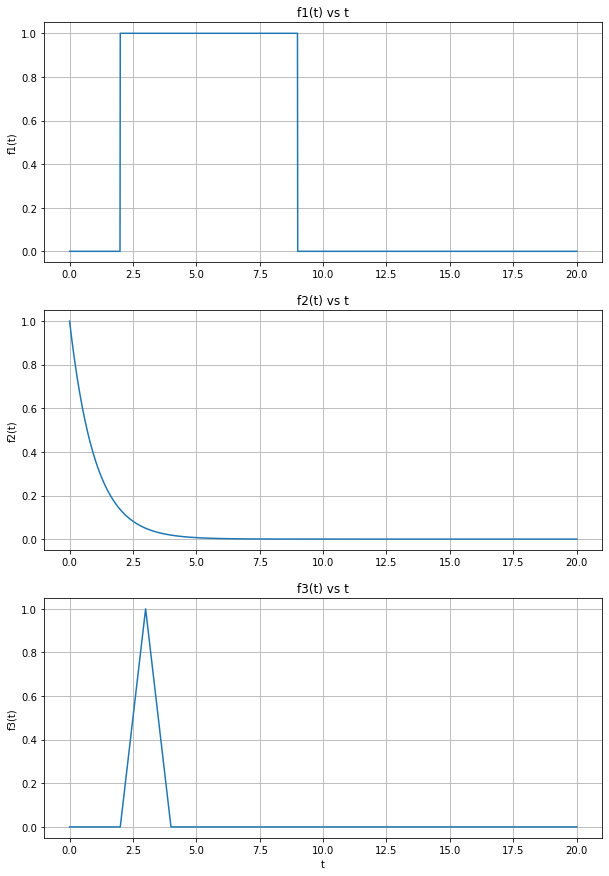
\includegraphics[scale=0.6]{functs 1-3.png}

    \paragraph{} As seen above, some of my expectations held true. The first function worked just as speculated, but I neglected to notice the negative exponent on the second function. So, I didn't expect the second function's negative slope, but it makes sense. For the final function, I was surprised to see such a steep peak. I was incredibly far off for the final function because I incorrectly distributed the outer functions when I tried calculating it out by hand.  

    \paragraph{} The second set of results for Lab 3 are the plots from Section 2, Parts 2-4, seen in the lab handout. These plots are essentially used to verify that our user-defined convolution function was created correctly through comparison to the library's convolution function. My expectation for these figures are that each figure's plots are the same. 
    
    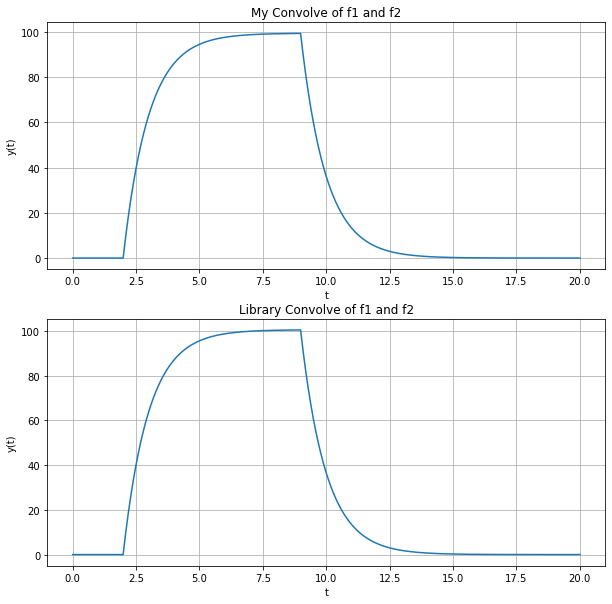
\includegraphics[scale=0.6]{task 2.png}

    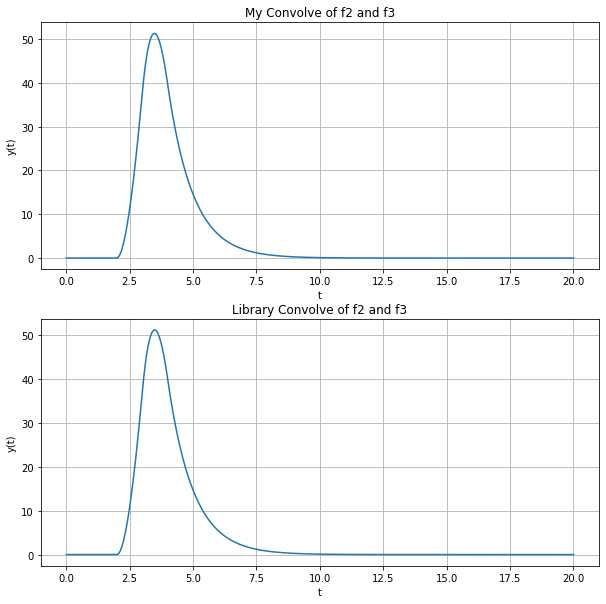
\includegraphics[scale=0.6]{task 3.png}

    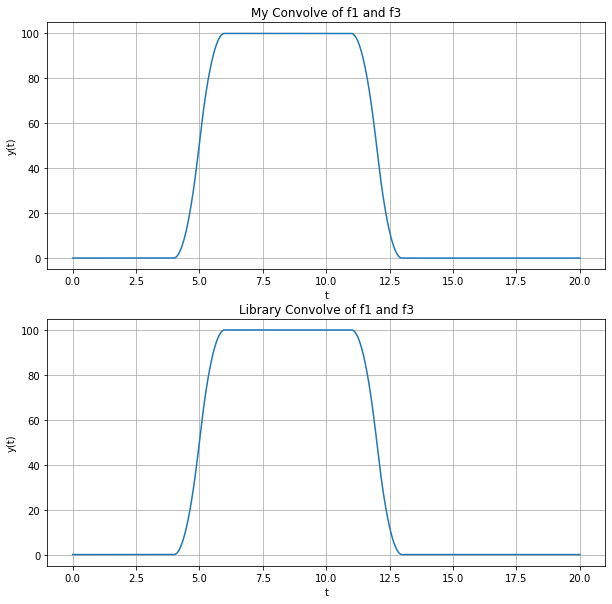
\includegraphics[scale=0.6]{task 4.png}

    \paragraph{} The library convolution and my user-defined convolution function gave the same resultant functions, so my expectation held true. Therefore, I can say with relative certainty that I constructed the convolution function correctly.  

\section{Error Analysis}

%This section will discuss error analysis of the experiment. Since this lab %deals with ideal simulation there shouldn't be any sources of error, so %instead this section can be used to describe any difficulties you had during %lab and how you solved them. Alternatively, if you couldn't get the %experiment to work, which is okay, you need to use this section to explain why %you couldn't get it to work to earn full points. 

\paragraph{} Some possible forms of error include: incorrect indexing and not making the time the resultant convoluted function is graphed over long enough. As seen in the code for the user-defined convolution function, there are several instances of subtracting 1 or two values to account for indexing beginning at zero. Missing just one of these could throw the whole function off and trip the 'exception' case. On that note, the try-except clause is a great way to catch errors and it was a useful tool during this lab. The resultant convoluted function needs to be graphed over a much longer time interval than its two input functions because of the previously mentioned property of 'Duration', so a possible form of error is not recognising this and incorrectly plotting the output from the Convolution function.

\section{Questions} %also address any deliverables not yet put in yet
    \begin{enumerate}
        \item Did you work alone or with classmates on this lab? If you collaborated to get to the solution, what did that process look like?
        \paragraph{} I worked mostly alone on this lab. I spent quiet a bit of time before the lab section researching convolution and its details. 
        \item What was the most difficult part of this lab for you, and what did your problem-solving process look like?
            \paragraph{} The greatest problem I encountered during lab 2 was trying to understand how the way we were computing the convolving of two functions lined up with the integral we'd been shown in class. Conceptually, this is very challenging material and required a great deal of deliberating. I was able to mostly overcome this problem with the drawn-out help from the TA in the lab. My process mostly involved writing out arrays, convolving them by-hand with help from examples, and trying to discern patterns. 
        \item Did you approach writing the code with analytical or graphical convolution in mind? Why did you chose this approach?
            \paragraph{} I tried both approaches, but neither made much sense to me without concrete examples. In the end, analytical convolution worked better for me since we needed to calculate the resultant function at each individual point. The analytical approach worked better for me because I understand analytical convolution better than graphical since it has a clearer method to solve in my opinion. 
        \item . Leave any feedback on the clarity of lab tasks, expectations, and deliverables.
            \paragraph{} The pseudo-code was helpful, but the comments were fairly ambiguous and abstract. They were easy to misinterpret and only really helped thinking about the general concept and once the TA wrote out the code in-lab. Everything else was rather clear-cut and well-done. 
    \end{enumerate}

\section{Conclusion}

%Discuss briefly what you learned in this lab and whether or not you feel the %lab was successful. Include any recommendations for future labs as this is a %learning experience for all of us. Discuss any insights you gained from this %lab and how that will affect future work. \textit{Note: The bibliograhpy %needs to be on its own page.}

    \paragraph{} From lab 2, I learned how to convolve functions through summation. Once again, I should spend less time on the lab before-hand because the TA helped immensely in understanding the requirements and the thought process behind summation convolution. I feel that receiving the lab days in advance helps mull over the concepts, but I need to control myself on putting too much time into implementing them too early. Overall, I feel like this lab was only somewhat successful since convolution is still a rather muddled concept for me. 

Github: \url{https://github.com/SethCram} 

\newpage

\end{document}